\documentclass{article}
\usepackage{graphicx}
\usepackage{hyperref}
\usepackage{url}

\setlength{\parskip}{1em}

\begin{document}


\title{Visualizing Output}

Currently, ICE features two plugins for visualizing and plotting simulation
output data:

\textbf{VisIt Tools} - An interactive visualization tool for rendering data
defined on 2D and 3D meshes.

\textbf{CSV Plotting Tools} - A customizable, 2D data plotting utility for data
in CSV format.

\section{Installation and Configuration}

The CSV Plotting Tools require no additional software or preparation before use.
The VisIt Tools need both a VisIt installation and a connection between ICE and
a VisIt session.

\subsection{VisIt Installation} 

Before preparing ICE,
\href{https://wci.llnl.gov/simulation/computer-codes/visit/}{VisIt} must be
downloaded and installed. The ICE development team recommends using the latest
version of VisIt but acknowledges that any version greater than or equal to
2.8.2 should work. VisIt does not need to be installed on the same machine where
ICE is installed since ICE is capable of launching a VisIt session on a remote
machine. Regardless of the host, make note of the directory where VisIt is
installed as it will be necessary in the next step.

\subsection{Configuring the VisIt Connection}

Once VisIt is installed, ICE must connect to a running instance of VisIt in
order to make use of its rendering capabilities. ICE provides two different
tools that utilize VisIt, the Plot Editor and the Visualization Perspective.
Both utilities provide slightly different functionality and are accessed
through different means.

\subsubsection{Connecting for the Plot Editor} 

The Plot Editor uses a default connection to VisIt established in the ICE
Preferences page. This process only needs to be performed once. After initially
creating the connection, ICE will launch and connect with VisIt upon each
subsequent launch of ICE.

To set the connection, select Window $\rightarrow$ Preferences\ldots in ICE's
menu bar. (On Mac OS X, Preferences\ldots is instead located under Eclipse
ICE in the menu bar.) Select Visualization $\rightarrow$ VisIt
in the tree on the left side of the Preferences window.

\begin{center}
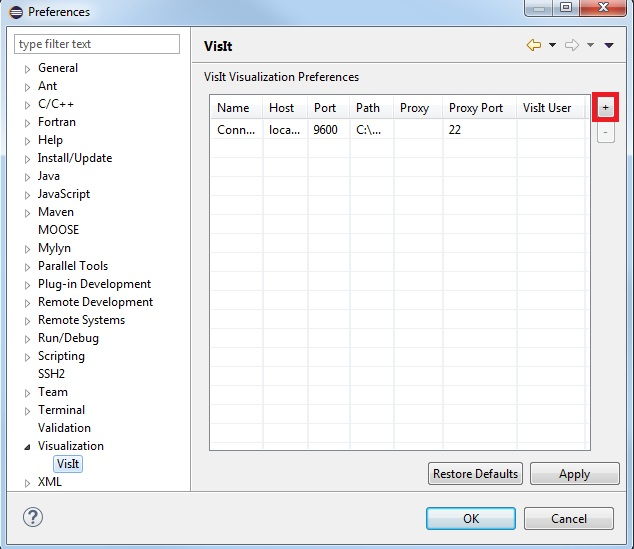
\includegraphics[width=12cm]{images/VisItPreferencePage_ICE}
\end{center}

Press the button with a ''+" symbol in the upper right (highlighted in the image
above) to add a new row to the table. Click on cells in the new row to edit
their values. The default values automatically supplied by ICE should be
appropriate for most users. However, two fields may need to be changed:

\textbf{Host:} The default value of ''localhost" allows for connections to VisIt
installations on the same machine where ICE is running. To launch a remote VisIt
connection, change this to the hostname of that machine.

\textbf{Path:} Enter the full path to the directory containing the VisIt
executable, not the executable itself. The VisIt executable is named
\textit{visit} on Linux and Mac OS X. On Windows, \textit{VisIt.exe} is the
appropriate file.

Once finished editing the cells in the new row, press Apply, then OK. ICE will
then launch an instance of VisIt and connect to it.

\subsubsection{Connecting for the Visualization Perspective} 

To establish a VisIt connection in the Visualization perspective, begin by
opening this utility. In the main menu bar at the top of the window, select
Window $\rightarrow$ Perspective $\rightarrow$ Open Perspective $\rightarrow$
Other\ldots. Select Visualization in the dialog that appears and click OK.
Alternatively, the same dialog may be accessed by clicking the Open Perspective
button in the toolbar in the upper right-hand corner of the ICE workbench.

\begin{center}
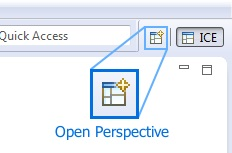
\includegraphics{images/ICE_OpenPerspective}
\end{center}

Click the Launch VisIt button in the tool bar to enter the VisIt connection
parameters.

\begin{center}
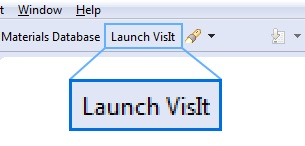
\includegraphics{images/ICE_VisItLaunchButton}
\end{center}

The resulting dialog offers three options for connecting to VisIt.

\begin{center}
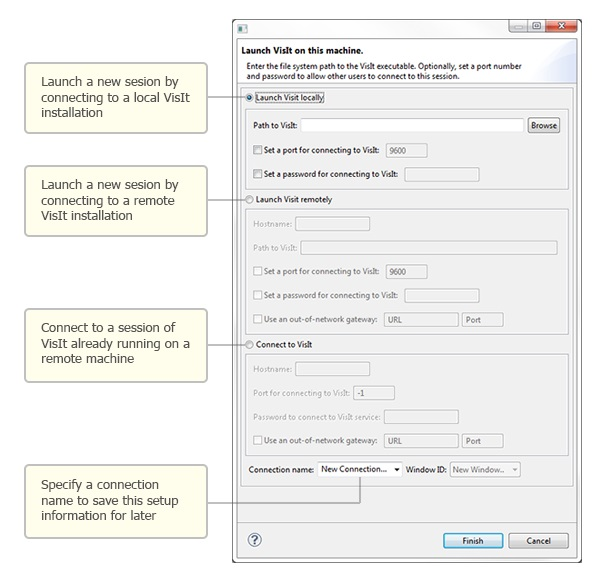
\includegraphics[width=12cm]{images/ICE_VisItLaunchOptions}
\end{center}

\textbf{1) Launch VisIt locally -} This connection option will launch a new
VisIt session on the machine running ICE. If VisIt in installed on this machine,
use the Browse button to enter the directory containing the VisIt executable
into the Path to VisIt field. Optionally, set a port number (default 9600) that
VisIt will use to serve data to ICE, and if this VisIt session will be shared
with multiple userd, set a password.

\textbf{2) Launch VisIt remotely -} Using this method of connecting will launch
a new VisIt session on a machine other than the one used to run ICE. Specify the
hostname and full path to the directory containing the VisIt executable.
Optionally, enter a port number (default 9600), and if VisIt session will be
shared with multiple users, enter a password. If access to the remote machine
where VisIt is installed requires the use of an external gateway or proxy,
specify its URL and port number, as well.

\textbf{3) Connect to VisIt -} To connect to a previously launched VisIt
session, specify the hostname, port number, and password set on the lanuch of
that session. This information will need to be obtained from the person who
initially launched the VisIt session. If access to the machine hosting the VisIt
session requires the use of an external gateway or proxy, enter its URL and port
number, as well.

For a reminder of where VisIt is installed on Windows, find a shortcut to
VisIt on the desktop or in the start menu. Right-click the shortcut and open its
Properties. The path to the VisIt executable's directoy will be shown next to
Target.

Regardless of the method used to connect to VisIt, enter a Connection
name at the bottom of the dialog. 

When connecting to an existing session, specify a Window ID between 1 and 16.
The Window ID used determines how ICE will connect to VisIt. If multiple users
connect using the same Window ID, they will all see and be able to interact with
the same VisIt view. However, if multiple users wish to each have their own
unique session with its own controls, assign a unique Window ID to each user.
The VisIt installation can support up to 16 unique window IDs at a time.

Once the required fields are complete, click the Finish button at the bottom,
and ICE should begin connecting to VisIt.

\section{VisIt}

\subsection{Opening a VisIt File}

\subsubsection{Opening a Plot Editor} 

To open a Plot Editor, a file that uses this editor must first be placed in the
Project Explorer. This view lists files imported into ICE. To access the Project
Explorer, use the the menu bar at the top of the window and navigate to Window
$\rightarrow$ Show View $\rightarrow$ Project Explorer. Depending on the active
Eclipse perspective, opening this view may require selecting Other\ldots and
finding the Project Explorer in the dialog under the General category in the
tree.

By default, the Project Explorer should automatically import the
ICEFiles/default and ICEFiles/itemDB folders. If it does not, or if you want to
import a different folder into ICE, right click in the Project Explorer and
select Import\ldots from the context menu. Then, select General $\rightarrow$
File System from the tree, and press the Next button. Select directories and/or
files to import into the Project Explorer, and enter which folder they should
be imported into, as shown below.

\begin{center}
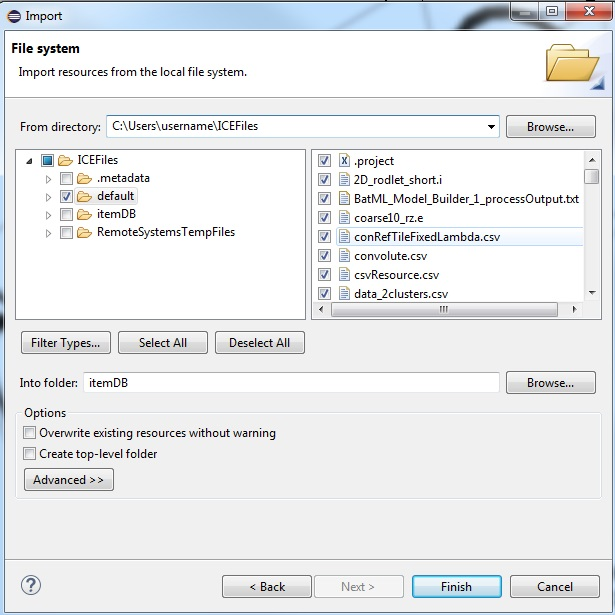
\includegraphics[width=12cm]{images/ImportFileDialog}
\end{center}

Once a file is in the Project Explorer, simply double click on it to open it in
VisIt.

\subsubsection{Opening in the Visualization Perspective}

\begin{center}
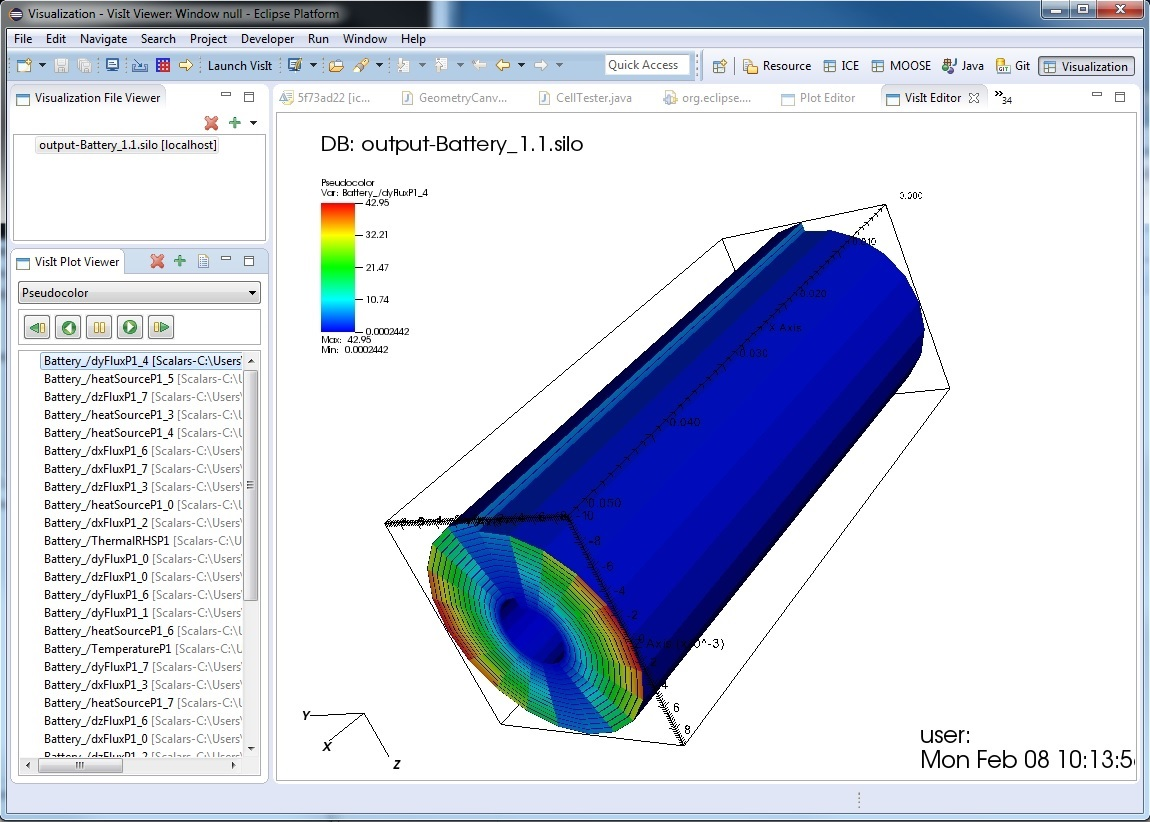
\includegraphics[width=12cm]{images/VisualizationPerspectiveOverview}
\end{center}

To open a file in the Visualization Perspective, first import the file into the
Visualization File Viewer, located in the upper left of the screen. Click the
Open a File button (green plus sign icon). The resulting dialog allows for the
selection of local files to import.

\begin{center}
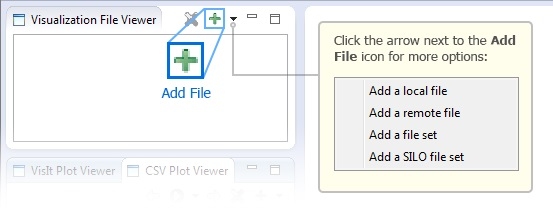
\includegraphics[width=12cm]{images/VisualizationAddFile}
\end{center}

Currently, ICE can only open files in VisIt on the same machine that is running
the VisIt session. For a connection to a remote VisIt installation, click the
arrow beside the Open a File button, and select ``Add a remote file'' from the
drop down menu. The resulting dialog box allows the user to browse the file
system of the remote machine hosting the VisIt session.

\begin{center}
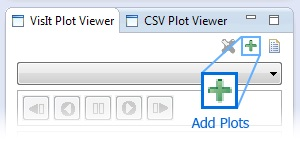
\includegraphics[width=12cm]{images/VisualizationAddPlots}
\end{center}

Once a file is in the Visualization File Viewer, create a plot by selecting the
file, and then clicking the Add a Plot to the List button located in the VisIt
Plot Viewer in the lower part of the column on the left side of the workbench.
The resulting dialog allows the user to select plots from the file to view.
After mading a selection or selctions and pressing OK, these plots will be
placed in the VisIt Plot Viewer.

\begin{center}
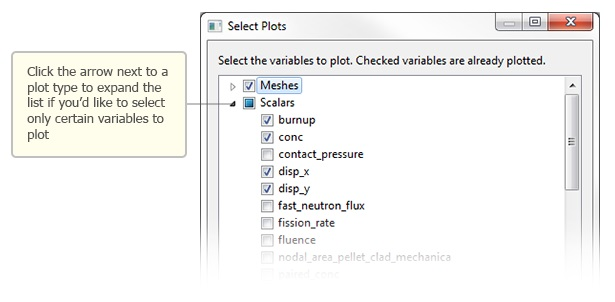
\includegraphics[width=12cm]{images/VisualizationSelectPlots}
\end{center}

Finally, double click a plot in the VisIt Plot Viewer to render the data to the
screen.

\subsection{Using VisIt}

Both the Plot Editor and the Visualization Perspective allow the user to rotate
the model by clicking and dragging inside the display area or adjust the zoom by
scrolling the mouse wheel. Other commands vary slightly between the two
utilities.

\subsubsection{Selecting the Plot}

In the Plot Editor, pressing the Select Series\ldots button will open a dialog
which lists the various plots in the opened file. Simply select one and click OK
to open it. 

\begin{center}
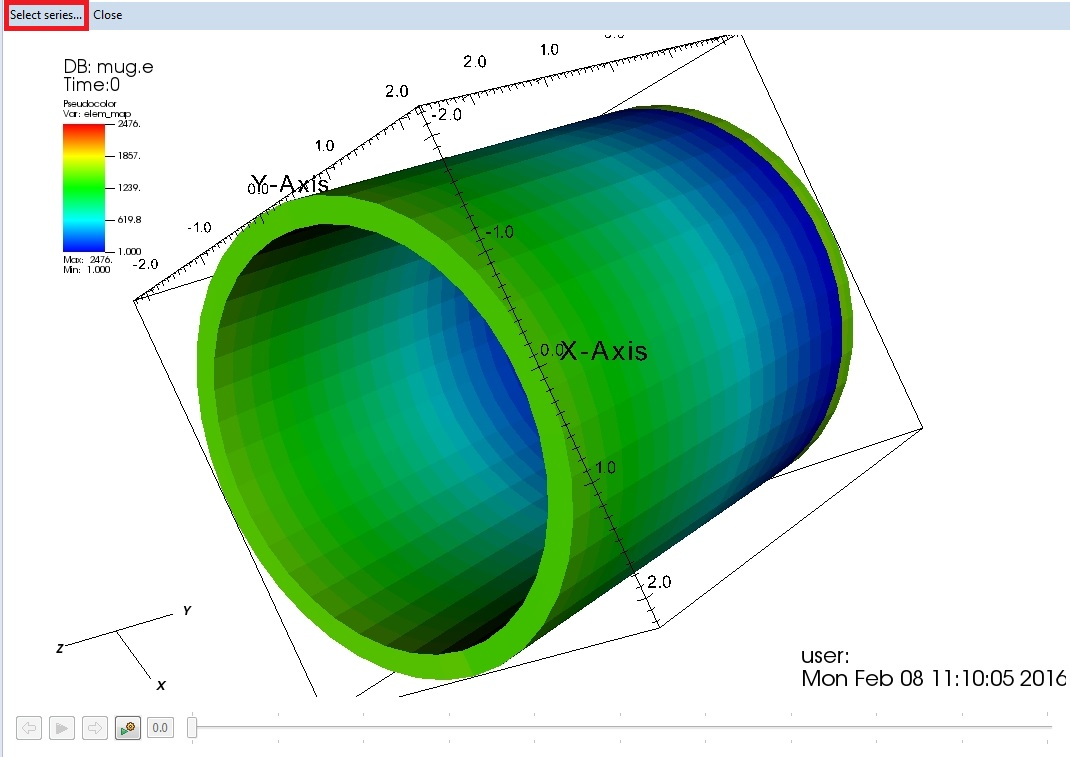
\includegraphics[width=12cm]{images/PlotEditorSelectSeriesButton}
\end{center}

In the Visualization Perspective, the opened plots will be listed in the VisIt
Plot Viewer. Double click on one to open it.

\subsubsection{Setting the Plot Representation}

VisIt is capable of displaying plots in several different representations, such
as pseudocolor, contour, or volume.

To switch between plot types in the Plot Editor, right click inside the display
area and select one of the listed options under the Representation category in the
context menu.

The Visualization Perspective features a drop down menu at the top of the VisIt
Plot Viewer which allows for switching between the available representations. 

\begin{center}
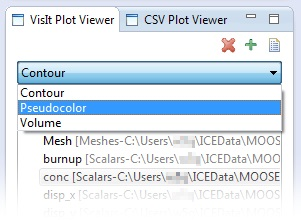
\includegraphics[width=12cm]{images/VisItRepresentationDropDown}
\end{center}

\subsubsection{Animation and Time Data}

The Plot Editor features a time slider widget at the bottom of the screen. 

\begin{center}

\includegraphics[width=12cm]{images/TimeSliderWidget}
\end{center}

The controls, in order of left to right, are:

1) Return to the previous time step.

2) Automatically play the plot as an animation by displaying the time steps
sequentially. 

3) Advance to the next time step. 

4) Opens an options menu that allows the user to set the playback speed, toggle
whether the animation should loop when it reaches the end, and set the plot to
the first or last time step.

5) A display for the current time step. It can be edited to set the plot to an
arbitrary time step. 

6) A slider that shows the current time step's position on the timeline. The
slider can be dragged around the timeline, setting the plot's time step
accordingly.

In the Visualization Perspective, the Visit Plot Viewer has a similiar set of
controls.

\begin{center}
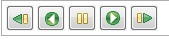
\includegraphics[width=12cm]{images/VizPerspectiveTimeControls}
\end{center}

The buttons, in order of left to right, are:

1) Return to the previous time step.

2) Automatically play the plot as an animation backwards, going through the time
steps in reverse order.

3) Pause the animation.

4) Automatically play the plot as an animation by displaying the time steps
sequentially.

5) Advance to the next time step. 

\subsubsection{Sending VisIt Python Commands}

This functionality is only available in the Visualization Perspective.

\begin{center}
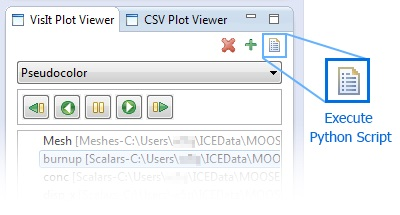
\includegraphics[width=12cm]{images/PythonScriptButton}
\end{center}

The Execute Python Script button in the upper right of the VisIt Plot Viewer
will open a new window with a Python shell. Commands entered into this shell
will be sent to the instance of VisIt. 

Python code can be written into the shell directly, but the Load from File
button will import an existing .py script into the console. Once done, hit the
Execute button to send the python command(s) to VisIt.

Writing Python scripts for VisIt is beyond the scope of this tutorial. Please
refer to the
\href{https://wci.llnl.gov/simulation/computer-codes/visit/manuals}{VisIt Python
Interface Manual} provided by the VisIt development team at Lawrence Livermore
National Laboratory for information on Python commands for VisIt.

\section{CSV Plot Viewer}

ICE offers functionality for the viewing of CSV files. 

\subsection{Opening a CSV File}

CSV files are opened in Plot Editors through the Project Explorer. Open the
Project Explorer with Window $\rightarrow$ Show View $\rightarrow$ Project
Explorer and import the file by right clicking and selecting import. Once the
file is in the Project Explorer, double click to open it.

ICE expects CSV files to be in an [m x n] format, with no row holding empty
values. The first row in the file will be used to name a series, with the series
data being specified by the column of values beneath it.

\subsection{Using the CSV Plot Viewer}

\begin{center}
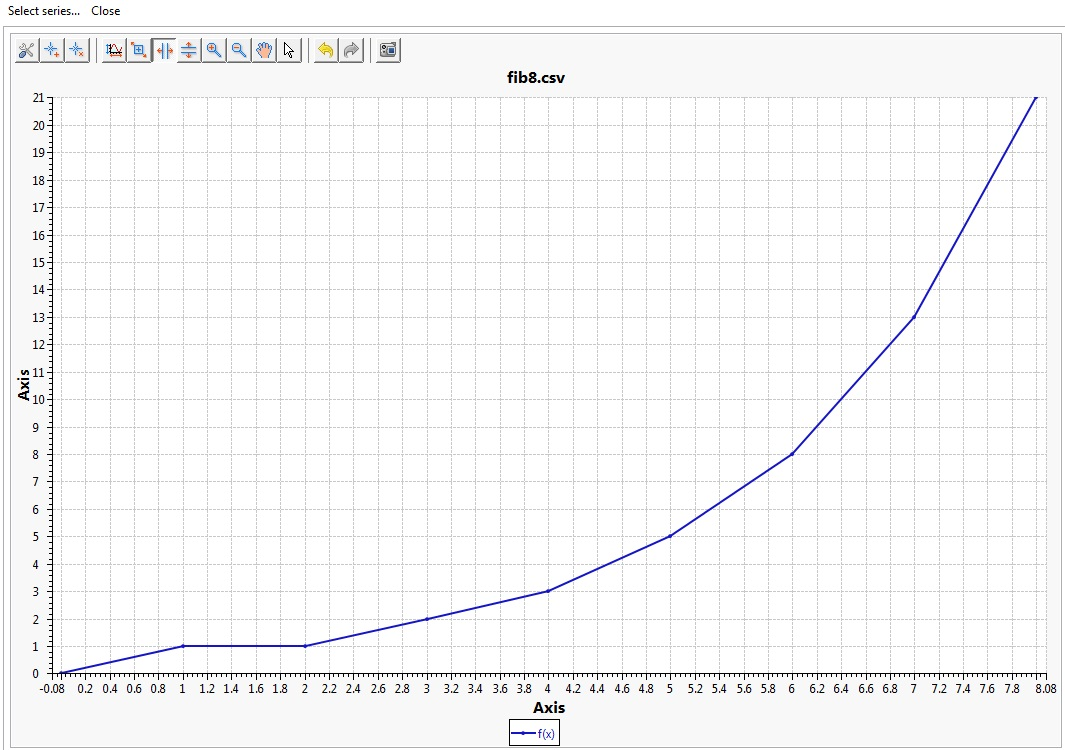
\includegraphics[width=12cm]{images/CSVPlotViewer}
\end{center}

\subsubsection{Controlling the Graphics}

The row of buttons at the top of the viewer provide basic graph editing
capabilities.

The first button allows the user to edit a variety of basic graph attributes,
such as font, axis titles and scales, line colors, etc.

The next two buttons allow for the addition and removal of annotations for
specific data points. 

The central grouping of buttons allow the user to zoom and pan the camera in a
variety of ways. 

The two yellow arrow buttons will undo/redo changes made to the graph.

The final button will export a screenshot of the graph.

\subsubsection{Setting the Independent Series}

By default, the first column in the file will serve as the independent series
setting the graph's x axis. By right clicking the Plot Viewer and selecting Set
Independent Series\ldots, the user can set the independent series to any other
series in the file.

\subsubsection{Setting the Dependent Series}

When first opened, only the series defined by the second column in the file will
be displayed. There are several ways to change this. 

The Select series\ldots button in the upper left hand corner will display a list
of all the series in the file. Selecting one and pressing OK will graph that
series and removing all others.

Right clicking and choosing Select series\ldots from the context menu will open
a dialog in which any of the available series may be selected. All selected
series will be graphed at once with deselected series removed.

Finally, the Remove all series option in the context menu will completely clear
the graph.

\subsubsection{Viewing the Data}

At the bottom of the editor is a series of tabs.

\begin{center}
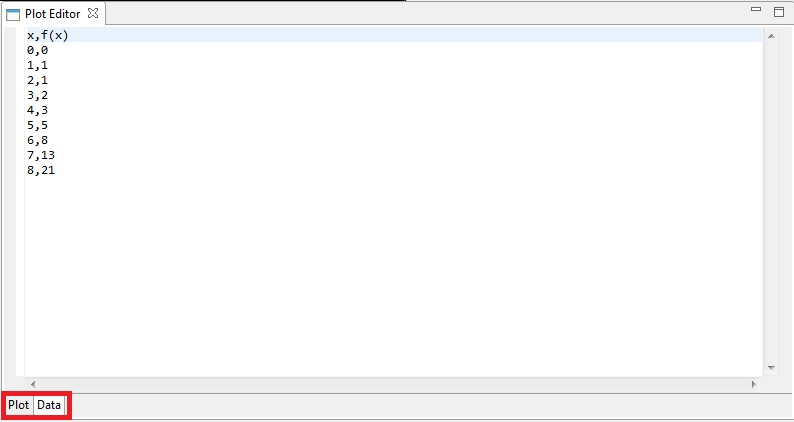
\includegraphics[width=12cm]{images/CSVTabs}
\end{center}

The Plot tab contains the graph described thus far. The Data tab will display
the raw numerical source data in a text editor. 

\section{MOOSE Embedded Visualization}

MOOSE Workflow Items allow for easy visualization of their associated files,
making use of the VisIt and CSV Plot Editors described previously.

\subsection{Creating a MOOSE Workflow}

First open the MOOSE Perspective, either through Window $\rightarrow$
Perspective $\rightarrow$ Open Perspective $\rightarrow$ Other\ldots and
selecting MOOSE, or by clicking the Open Perspective button in the top right
corner and selecting MOOSE.

\begin{center}
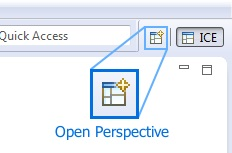
\includegraphics{images/ICE_OpenPerspective}
\end{center}

Next, you must open a MOOSE Workflow. The two buttons outlined in red below will
create Items. The upper one will import a .i file, while the bottom button will
create a new workflow. In either case, select MOOSE Workflow from the menu and
hit OK.

\begin{center}
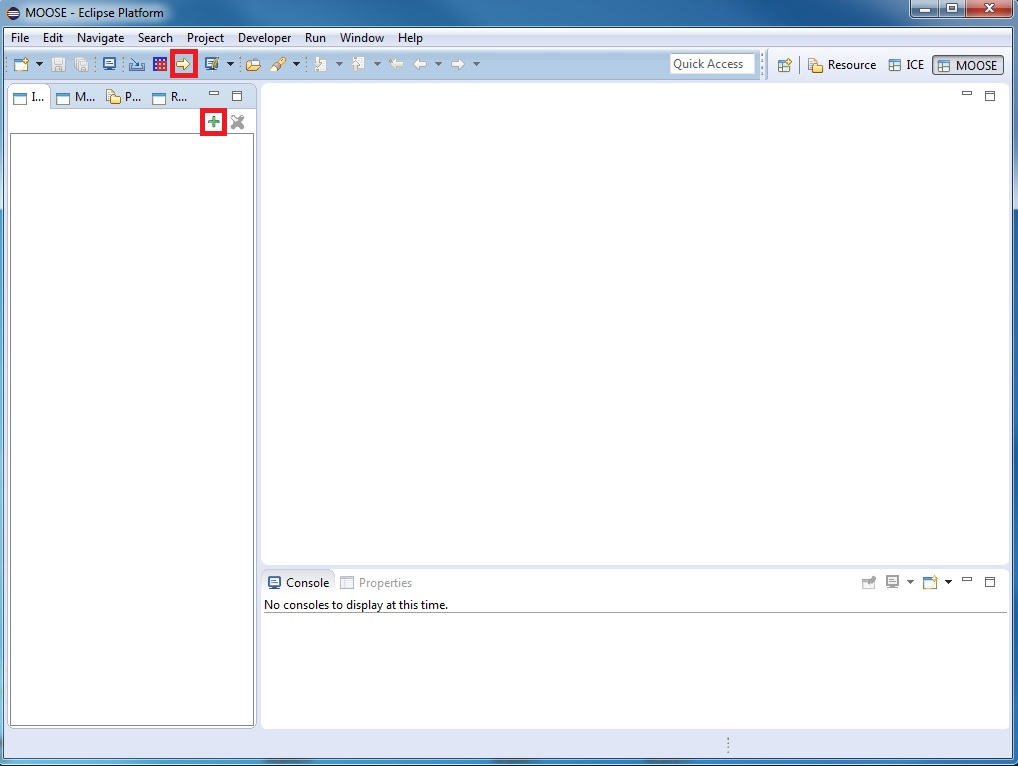
\includegraphics[width=12cm]{images/MOOSEPerspectiveNewWorkflow}
\end{center}

You must now choose the MOOSE application which will run the file. The
Browse\ldots button under MOOSE-Based Application in the upper left hand corner
will open a menu asking if the application is on the local machine or on a
remote one. For local applications, you will simply need to select it from a
dialog. 

\begin{center}
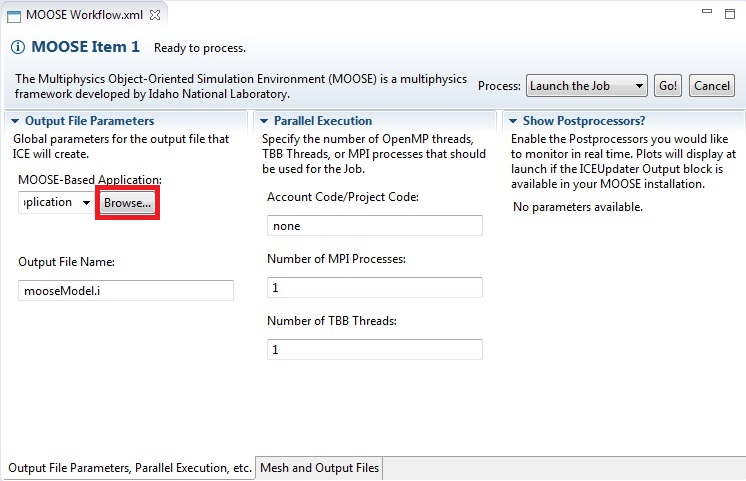
\includegraphics[width=12cm]{images/MOOSEItem}
\end{center}

If the application is remote, a new dialog will open. At the top, press the New
button to set up your connection. 

\begin{center}
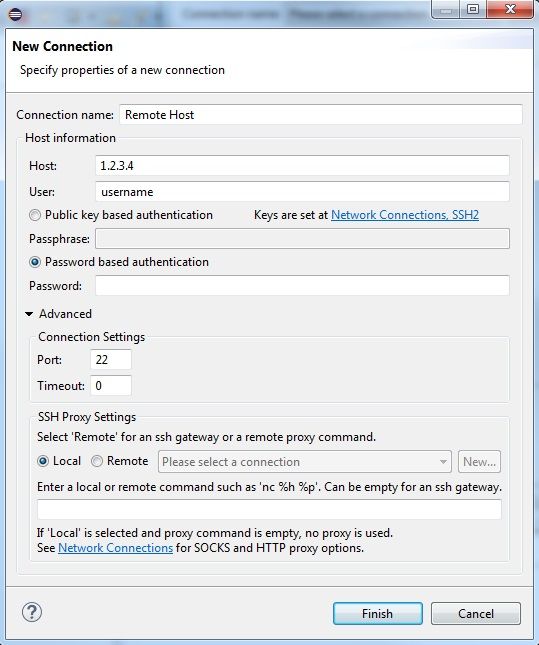
\includegraphics[width=12cm]{images/NewConnectionDialog}
\end{center}

You must set the Host to the computer containing the MOOSE application, and User
and Password to the username and password for your account on that machine. You
may also optionally set the Port number, timemout, and proxy settings. Once
done, click Finish. You will automatically be shown the file system for your new
connection. Select the MOOSE application from it and click OK.

Save the form. If you imported a file, there will still be unsaved changes after
a single save. You can save again and skip the next section. 

\subsubsection{Configuring the MOOSE Input Data}

\begin{center}
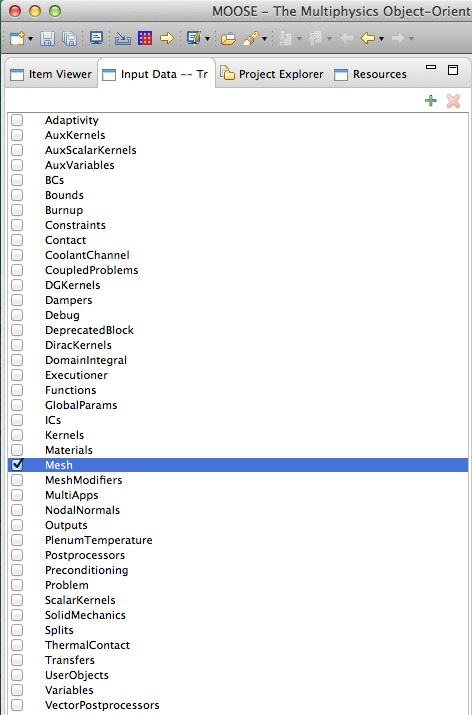
\includegraphics[width=6cm]{images/MOOSETree} 
\end{center}

If you did not import a pre-written MOOSE file, some setup will be
required before the job can create visualizations. Switch to the Input Data --
Tree View tab on the left of the screen. Here you will see a list of MOOSE data
categories. Click Mesh and switch to the Properties tab at the bottom.

\begin{center}
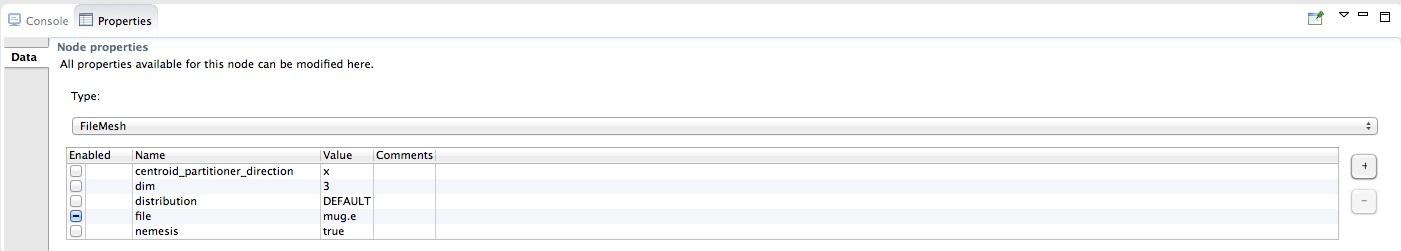
\includegraphics[width=12cm]{images/MeshProperty} 
\end{center}

The Properties tab will display the properties of the Mesh variable. At the top
will be drop down menu labeled Type. Select FileMesh from it and the table below
it will be populated. In the table, select the file line and place the file
containing the mesh you want to work with in it, as mug.e is in the example
above.

If there are any variables you want to graph from the job, you will have to
specify them as Variables and create PostProcessors which point to them,
similar to how you just set the Mesh. 

\subsection{Viewing the Embedded Visualizations} 

Once your MOOSE Workflow is set up, make sure the Process control is set to
``Launch the Job", and click the Go! button in the upper right hand corner. Wait
until the console shows that the output files are finished downloading, similar
to what is seen here:

\begin{center} 
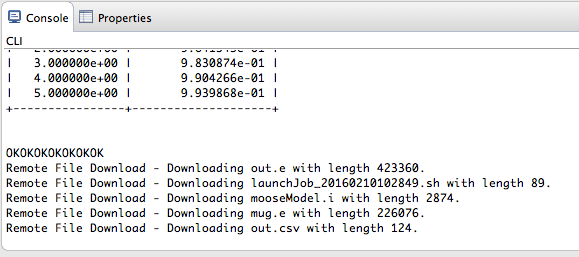
\includegraphics[width=12cm]{images/MOOSEJobConsoleOutput} 
\end{center}

You can now change to the Resources tab on the left. This will list all the
output files produced by the MOOSE job. Double clicking on one will open a Plot
Editor inside the MOOSE Item's Mesh and Output Files tab. The visualization can
be controlled normally, as described in previous sections.  

Multiple resources can be opened at once. At the top of the screen are controls
for the number of rows and columns making up the grid. These can be changed to
set the layout for the various plots, as demonstrated below.

\begin{center}
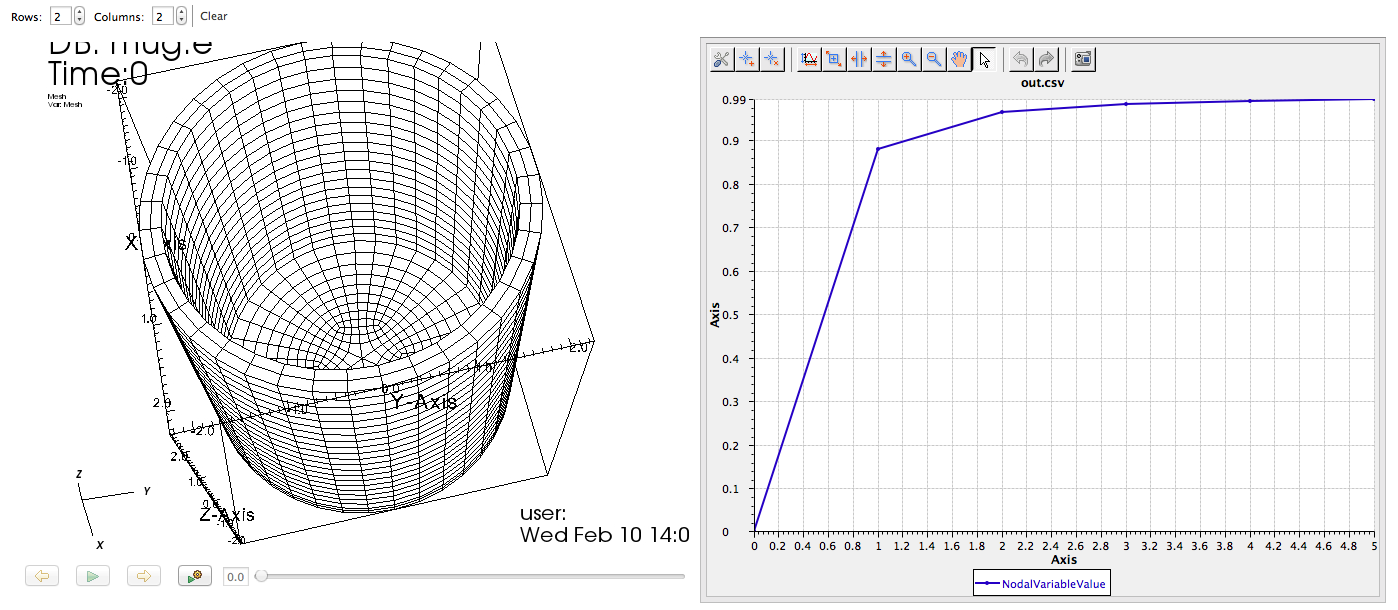
\includegraphics[width=12cm]{images/MOOSEEmbeddedHorizontal}
\end{center}

\begin{center}
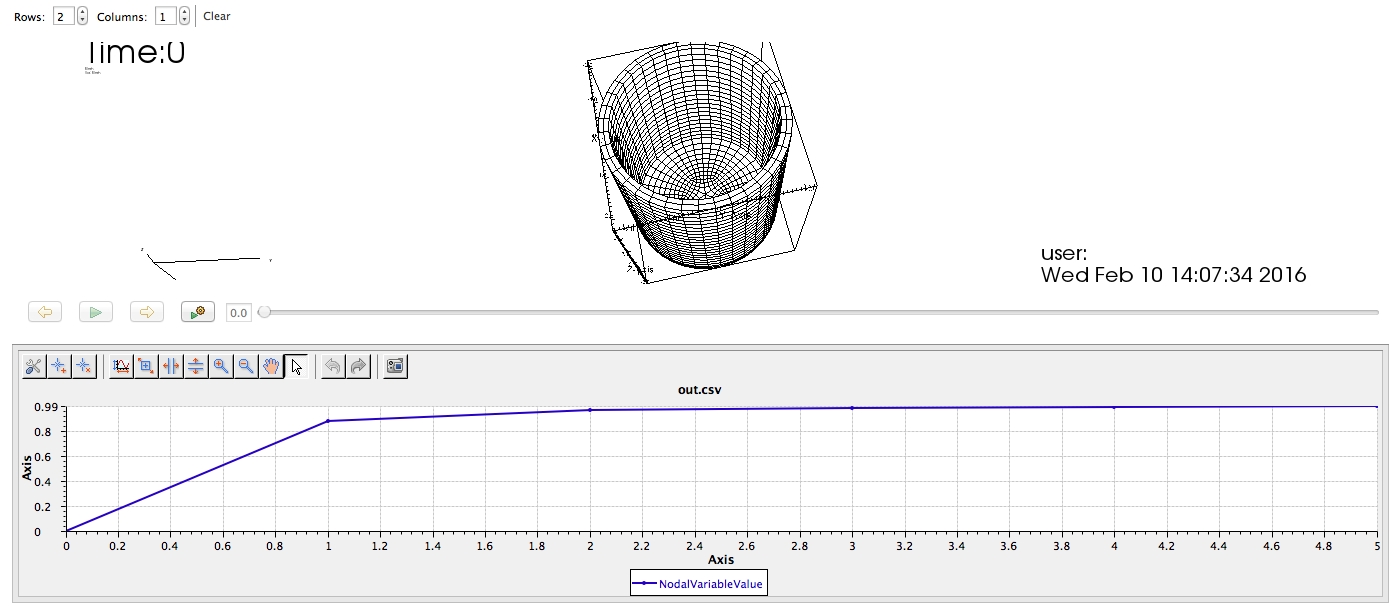
\includegraphics[width=12cm]{images/MOOSEEmbeddedVertical}
\end{center}

Be careful when reducing the number of rows or columns, as any plots which no
longer fit in the grid will be closed.

If you hover over a plot, a button will appear in the upper left hand
corner. Clicking it will close that plot.

\begin{center}
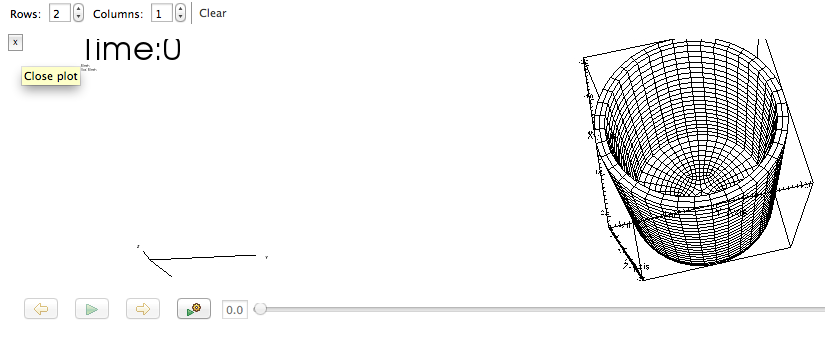
\includegraphics[width=12cm]{images/ClosePlotButton}
\end{center}

Alternatively, the Clear button next to the controls for the number of rows and
columns will close all the plots.

\end{document}

